\documentclass[final,hyperref={pdfpagelabels=false}]{beamer}
\usepackage{grffile}
\mode<presentation>
  {
  %  \usetheme{Berlin}
  \usetheme{I6pd2}
  }
  \usepackage{times}
  \usepackage{amsmath,amsthm, amssymb, latexsym}
  \boldmath
  \usepackage[english]{babel}
  \usepackage[latin1]{inputenc}
  \usepackage[orientation=portrait,size=custom,width=80,height=120,scale=1.4]{beamerposter}  
  
  % my packages
  
  %%%%%%%%%%%%%%%%%%%%%%%%%%%%%%%%%%%%%%%%%%%%%%%%%%%%%%%%%%%%%%%%%%%%%%%%%%%%%%%%%5
  \graphicspath{{figures/}}
  \title{Optimizing Simulink\textsuperscript{\textregistered} Models}
  
  \author{Bentley James Oakes}
  
  \institute[McGill University]{McGill University, Montreal, Canada}
  
  \date{\today}


  %%%%%%%%%%%%%%%%%%%%%%%%%%%%%%%%%%%%%%%%%%%%%%%%%%%%%%%%%%%%%%%%%%%%%%%%%%%%%%%%%5
  \begin{document}
  \begin{frame}{}
      
        \begin{block}{\large Problem Statement}
        \small
   		The Simulink\textsuperscript{\textregistered} modelling tool is used to diagram and study cyber-physical systems. One advantage
   		of modelling the systems in this way is that embeddable code can generated from the models directly.
   		However, this process means that inefficiencies in the model may be propagated to the code. Optimizations may be performed during code
   		generation, but this may lead to an unacceptable loss of traceability in determining
   		which parts of the model were modified or removed.\\~\\
   	    Our works focuses on defining model-to-model optimizations, where the optimized
   		model can be loaded back into Simulink for further development or analysis. We suggest this improves traceability and
   		can allow model specialization for different platforms. In this work, we present three optimizations to improve model simulation performance or the visual layout of the model.
        \end{block}
        

    \begin{block}{Optimization Classification}
    \begin{center}
    \small
    In our work, we propose an optimization classification based upon the platform-dependence and intent of the optimization. This classification creates
    stronger theoretical connections to the compiler domain and the model
    transformation field, and assists us to discover and implement new optimizations.
    \end{center}
    \vspace{-1.5cm}
            \begin{columns}[t,totalwidth=\linewidth]
             \begin{column}{.19\linewidth}
             \small
           \begin{center}\textbf{Model-level}\end{center}
           \footnotesize
           These optimizations are those that are not dependent in any way on the target architecture, and focus on changing the structure itself of the model. \\~\\~\\
           
           \textbf{Examples:}
           
           \begin{itemize}
           \footnotesize
           \item Algebraic simplification - Reduce computational effort
           \item Dead-block removal - Extraneous blocks should be removed
           \item Flattening - Remove subsystems from the model
           \end{itemize}
           
           \end{column}
           \hspace{-1.2cm}\vrule\hspace{.05cm}
           \begin{column}{.19\linewidth}
           \small
          \begin{center}\textbf{Platform-independent}\end{center}
          \footnotesize
            These optimizations are specific to a general class
            of target architecture, such as whether the target is single- or multi- core, or the
            target programming language of code generation. \\~\\
                       
           \textbf{Examples:}
           
           \begin{itemize}
           \footnotesize
           \item Transforming floating point calculations into integer representations
           \item Specializing blocks into structures appropriate for a given target language.
           \end{itemize}
            \end{column}
            \hspace{-1.2cm}\vrule\hspace{.05cm}
            \begin{column}{.16\linewidth}
            \small
          \begin{center}\textbf{Platform-dependent}\end{center}
          \footnotesize
            Platform-dependent optimizations can be characterized by their dependence on a particular target
            architecture.\\~\\
                                   
           \textbf{Examples:}
           
           \begin{itemize}
           \footnotesize
           \item Re-order blocks to account for machine's caching strategy
           \item Schedule blocks among machine's processors
           \end{itemize}
            \end{column}
            \hspace{-1.2cm}\vrule\hspace{.05cm}
            \begin{column}{.18\linewidth}
            \small
          \begin{center}\textbf{Optimization Hierarchy}\end{center}
          \footnotesize
            These classification levels can be placed in a hierarchical relationship, with optimizations
            further down the hierarchy more specific to a particular machine. \\~\\A code synthesis workflow may include transformations between these levels, so that a general model is specialized further and further until code is generated from a platform-specific model.
            \end{column}
            
            \begin{column}{.20\linewidth}
          ~\\~\\
            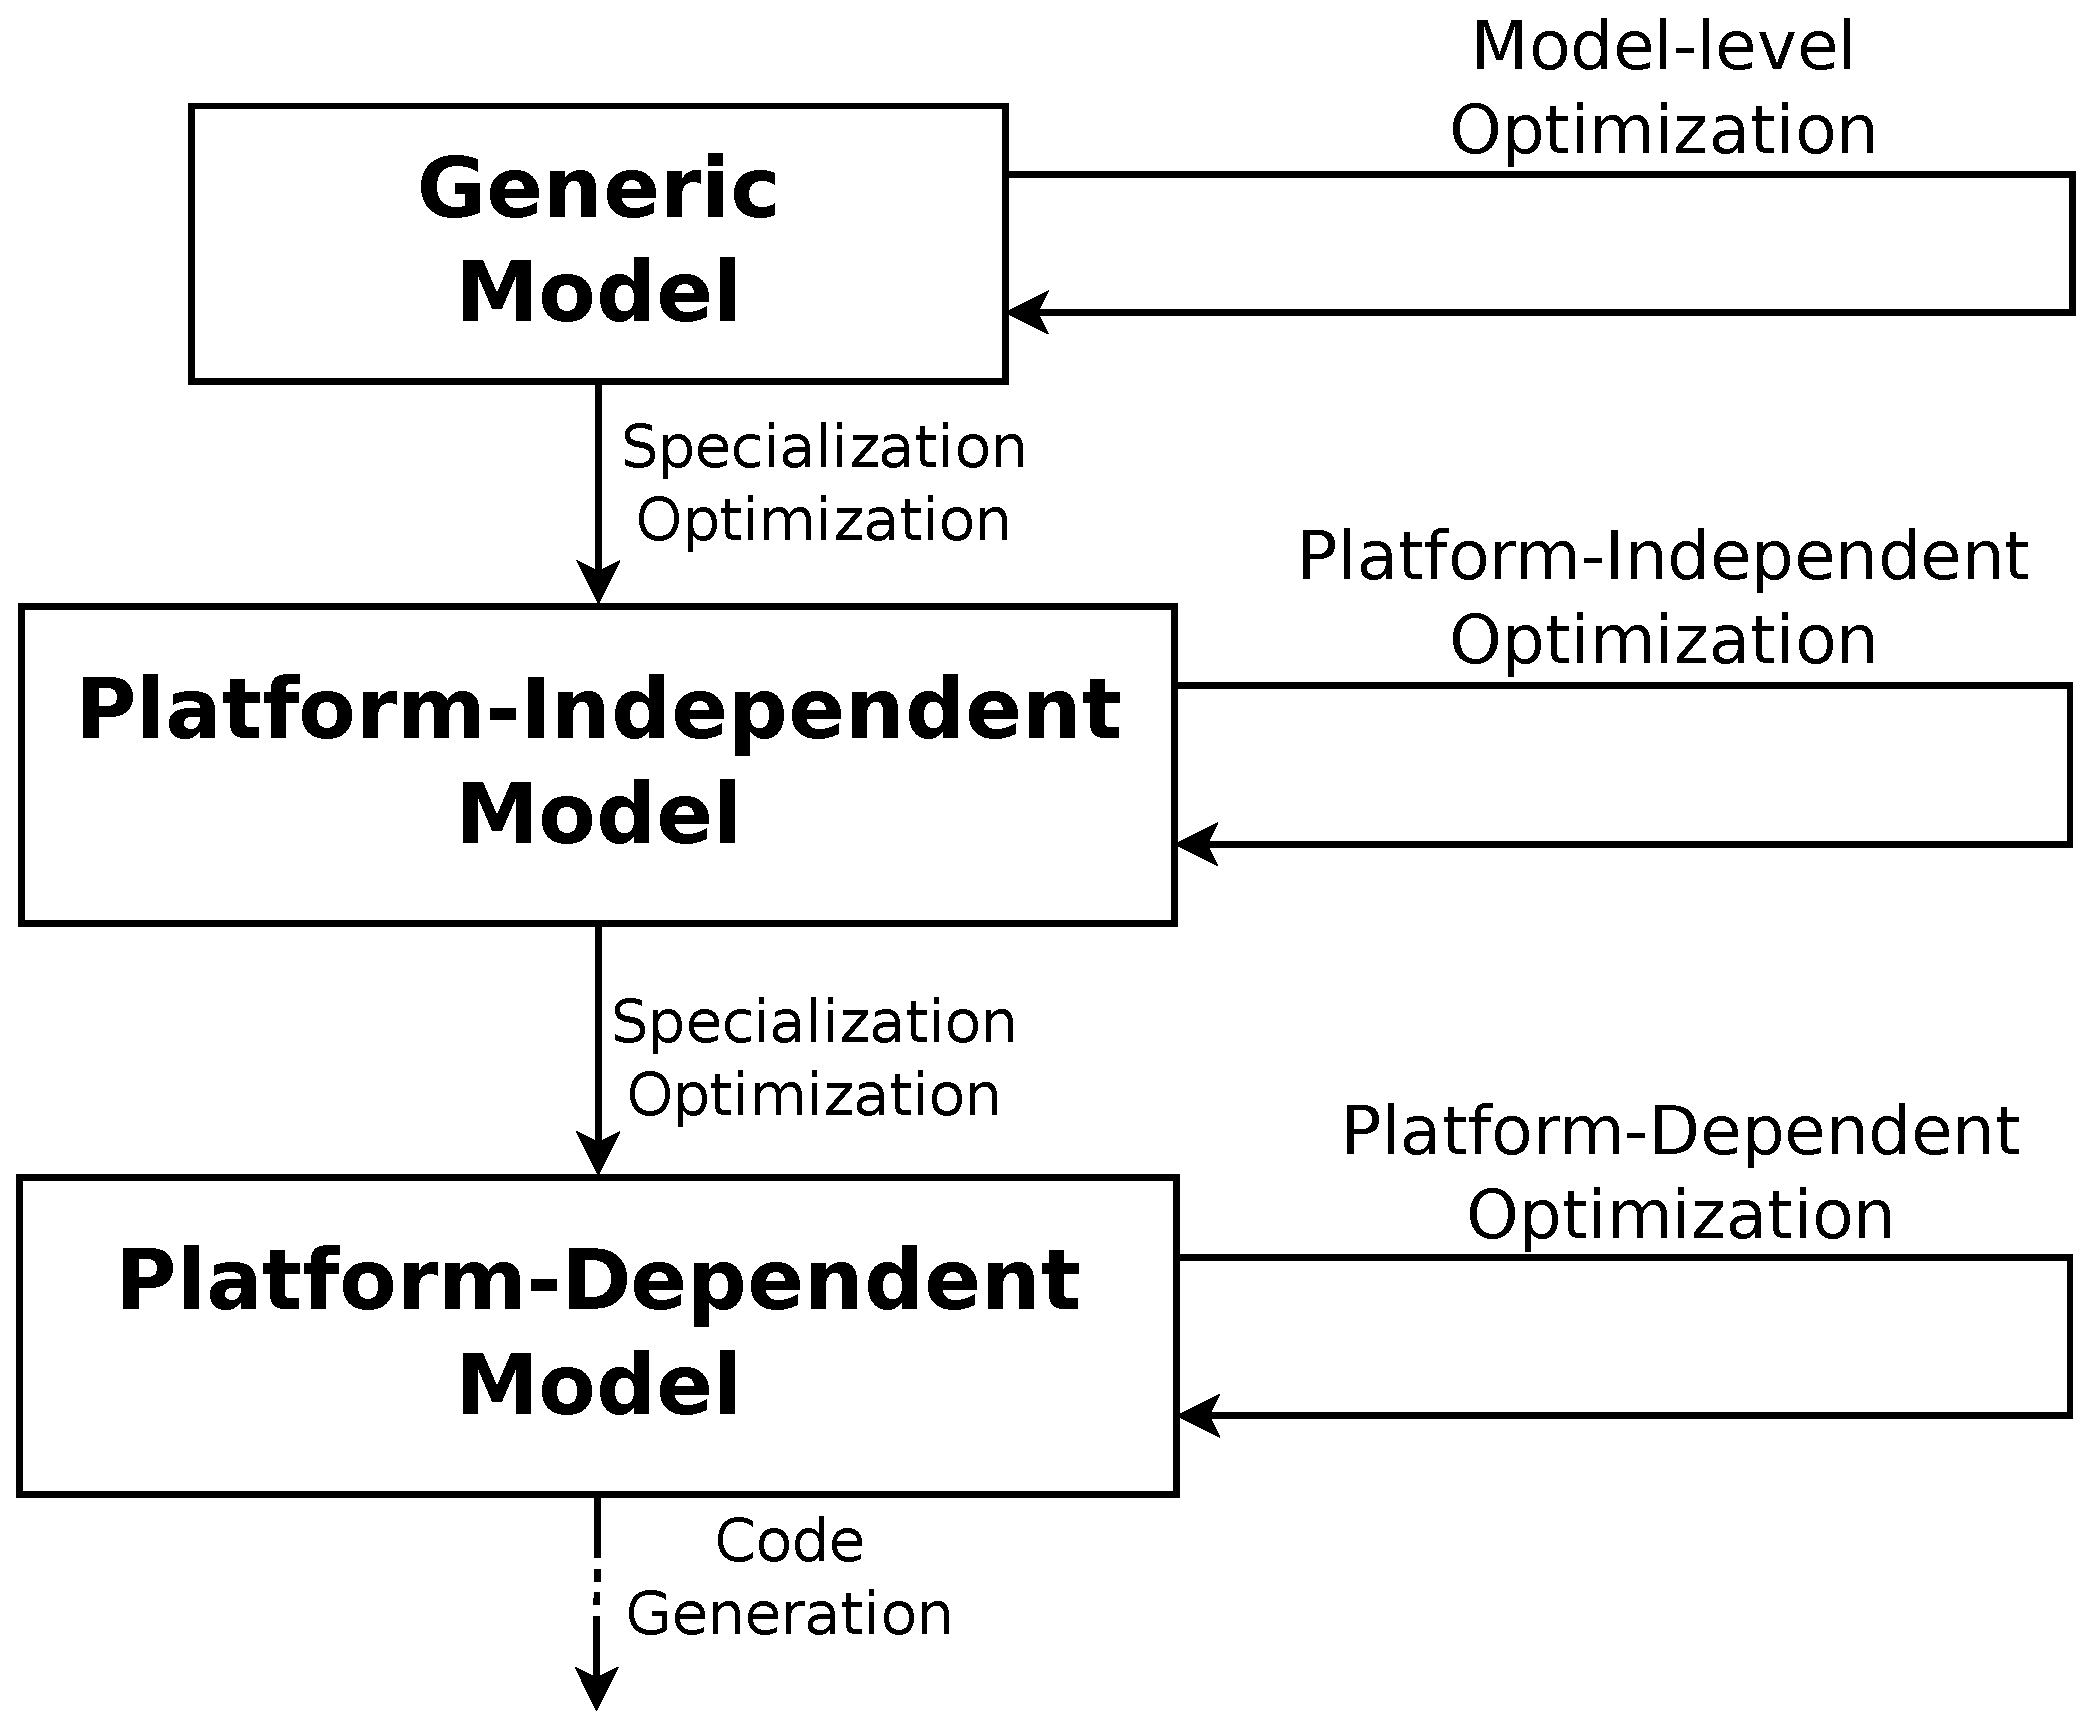
\includegraphics[width=\textwidth]{images/hierarchy}
            \end{column}
                        
                  \end{columns}
            \end{block}
	
        \begin{block}{Optimization Procedure}
        \vspace{-1.5cm}
        \begin{columns}[t,totalwidth=\linewidth]
         \begin{column}{.485\linewidth}
         \vspace{-.8cm}
         \small
       \begin{center}\textbf{Analysis}\end{center}
       \footnotesize
       Our work defines an analysis procedure to collect dataflow information for each node in the Simulink model. This procedure is based upon that used in the compiler literature. For example, for constant folding, the information propagated is whether a block will always produce a constant value during simulation.
       \end{column}
       \begin{column}{.485\linewidth}
       \vspace{-.8cm}
       \small
      \begin{center}\textbf{Transformation}\end{center}
        \footnotesize
        The optimization framework can then transform the model, based on the analysis results. This transformation is performed by utilizing the Himesis model format. After the transformation is complete, the optimized model is imported back into Simulink to be further developed.
        \end{column}
              \end{columns}
        \end{block}
      
      \vspace{-1.5cm}
    \begin{columns}[t,totalwidth=\linewidth]
    \centering
      \begin{column}{.585\linewidth}
        \begin{block}{Example Model-level Optimizations}
         \vspace{-.8cm}
        \small
        \begin{center}\textbf{Constant Folding}\end{center}
        \vspace{-0.3cm}
        \begin{columns}[c,totalwidth=\linewidth]
        \begin{column}{.485\linewidth}
        \begin{center}
        
        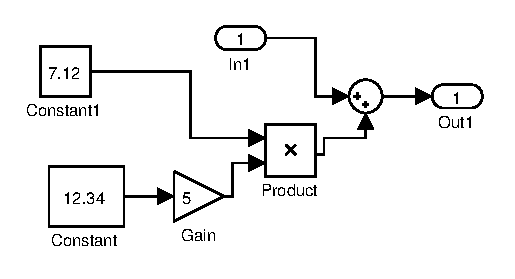
\includegraphics[width=0.8\linewidth]{images/models/Const1}\\
        \footnotesize \textit{Model before}
        \end{center}
        \end{column}
        \begin{column}{.485\linewidth}
        \begin{center}
        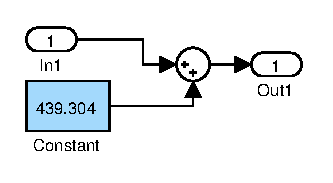
\includegraphics[width=0.7\linewidth]{images/models/Const1_export}\\
        \footnotesize \textit{Model after}
        \end{center}
        \end{column}
        \end{columns}
        \footnotesize ~\\~\\
        The constant folding optimization determines which blocks will always produce a constant value. For example, the four blocks on the left in the original model can be replaced by one constant block. This reduces the computational effort required to simulate this model.
         ~\\~\\
         \hrule
         
         \small
          \begin{center}\textbf{Dead-Block Removal}\end{center}
                 \vspace{-0.3cm}
         \begin{columns}[c,totalwidth=\linewidth]
         \begin{column}{.485\linewidth}
         \begin{center}
         
         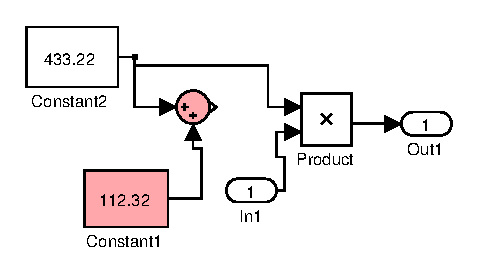
\includegraphics[width=0.8\linewidth]{images/models/HSimpleConstDead}\\
          \footnotesize \textit{Model before}
         \end{center}
         \end{column}
         \begin{column}{.485\linewidth}
         \begin{center}
         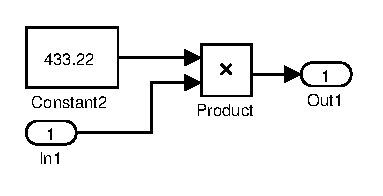
\includegraphics[width=0.8\linewidth]{images/models/HSimpleConstDead_export}\\
        \footnotesize \textit{Model after}
         \end{center}
         \end{column}
         \end{columns}
          \footnotesize ~\\~\\
         The dead-block removal optimization determines which blocks produce an output that is not further used in the model. For example, the output of the addition block on the left in the original model is not connected to another block. Thus the addition block and one constant block can be removed from the model.
          ~\\~\\
         \hrule
         \small
          \begin{center}\textbf{Flattening}\end{center}
                 \vspace{-0.3cm}
         \begin{columns}[c,totalwidth=\linewidth]
         \begin{column}{.485\linewidth}
         \begin{center}
         
         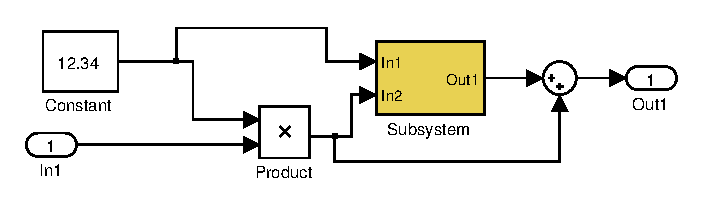
\includegraphics[width=0.8\linewidth]{images/models/Flatten1}\\
         \footnotesize \textit{Model before}
         \end{center}
         \end{column}
         \begin{column}{.485\linewidth}
         \begin{center}
         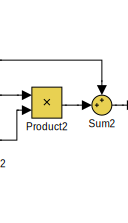
\includegraphics[width=0.6\linewidth]{images/models/Flatten1_subsystem}\\
         \footnotesize \textit{Inner subsystem before}
         \end{center}
         \end{column}
         \end{columns}
         \begin{center}
          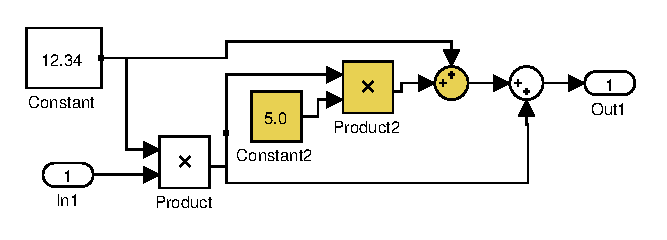
\includegraphics[width=0.5\linewidth]{images/models/Flatten1_export}\\
          \footnotesize \textit{Flattened model after}
          \end{center}
         \footnotesize
         The flattening optimization ``lifts'' blocks out of an inner subsystem of a model. Similarly to function inlining, this may allow further optimizations to further simplify the model. As well, a flattening transformation may replace the flattening step performed during code generation, allowing the code generator to be less complex.
         
        \end{block}
      \end{column}
\vspace{0.1cm}
     \begin{column}{.4\linewidth}
             \begin{block}{Experiments}

             \begin{table}[h]
             \footnotesize \textit{Simulation timings before and after model optimization}\\
             \centering
             \begin{tabular}{l | c c p{1cm} c c }
             
             \textbf{Optimization} &\multicolumn{2}{c}{\textbf{Before Opt. (sec.)}}& &\multicolumn{2}{c}{\textbf{After Opt. (sec.)}} \\
              & \textbf{Avg.} & \textbf{Std. Dev.} && \textbf{Avg.} &\textbf{Std. Dev.}\\\hline
              
             \textit{Constant Folding} & & & & & \\
             Model 1 & \textbf{19.78} &.05 && \textbf{16.95} & .21\\
             Model 2 & \textbf{18.35} & .07 &&\textbf{ 15.89} & .13\\
             Model 3 &\textbf{ 23.53} & .09 && \textbf{20.77} & .09\\
             Model 4 & \textbf{18.01} & .09 && \textbf{17.22} & .23\\
              & & && & \\
             \textit{Dead-Block Removal} & && & & \\
             Model 1 & 16.79 & .27 && 16.91 & .25\\
              & & && & \\
             \textit{Flattening} & & && & \\
             Model 1 & 18.87 & .22 && 18.75 & .19\\
             Model 2 & 21.77 & .16 && 21.75 & .38\\
             Model 3 & 19.54 & .12 && 19.94 & .06\\
             
             \end{tabular}
             \centering
             
             \end{table}
             
             \begin{table}[h]
             \footnotesize \textit{Timings for each step in our framework}\\
	          \centering
	          \begin{tabular}{l | c c }
	          
	          \textbf{Experiment Step} & \textbf{Avg. Time (sec.)} & \textbf{Std. Dev.} \\\hline
	           
	          Connect to Simulink & 11.71 & .24 \\
	          Import from Simulink & 4.94 & .04 \\
	          Create model in Python & .08 & .01 \\
	          Analysis & .02 & .00 \\
	          Transformation & .01 & .00 \\
	          Export to Simulink & .01 & .01 \\
	          
	          
	          \end{tabular}
	          
	          \end{table}
             \end{block}
             \vspace{-0.2cm}
             \begin{block}{Conclusions \& Future Work}
             \small
        	   The optimizations shown here demonstrate how the performance of a model simulation can be increased (as for the constant folding optimization), and how a model can be made visually simpler (as with the dead-block removal and flattening optimizations). Our framework allows these optimizations to be specified and implemented easily, and for a model to be optimized 
        	   
        	   ~\\
        	   Future work will focus on specifying more optimizations at all levels of the optimization hierarchy. As well, experiments will be performed on larger and more complex models. Finally, we aim to formally verify the model transformations used.\\~\\
        	   \footnotesize
        	   \textbf{Acknowledgments}\\
        	   We would like to thank Joachim Denil, Bart Pussig, and Pieter Mosterman from The Mathworks for their support.
             \end{block}
             \vspace{-0.2cm}
             \begin{block}{Bibliography}
             \small
     	   \begin{thebibliography}{10} 
     	   \bibitem{SLE2010} Bentley James Oakes, {\em Optimizing Simulink Models}, Report for COMP 621 - Program Analysis and Transformations, \url{https://github.com/BentleyJOakes/BDOT}
          		\end{thebibliography}	   
              	\end{block}
                     
                     
           \end{column}

    \end{columns}

  \end{frame}
\end{document}